\documentclass[12pt,a4paper]{article}

% ── Packages ──────────────────────────────────────────────────────────
\usepackage[utf8]{inputenc}
\usepackage[T1]{fontenc}
\usepackage{amsmath,amssymb,amsfonts}
\usepackage{mathtools}
\usepackage[authoryear,round]{natbib}
\usepackage{graphicx}
\usepackage{booktabs}
\usepackage{tabularx}
\usepackage{multirow}
\usepackage{float}
\usepackage{setspace}
\usepackage[margin=1in]{geometry}
\usepackage{hyperref}
\usepackage{caption}
\usepackage{subcaption}
\usepackage{array}
\usepackage{dcolumn}
\usepackage{threeparttable}
\usepackage{placeins}

\hypersetup{colorlinks=true, linkcolor=blue, citecolor=blue, urlcolor=blue}

\doublespacing

\newcolumntype{d}[1]{D{.}{.}{#1}}

% ── Title ─────────────────────────────────────────────────────────────
\title{\textbf{Sell in May and Go Away: \\ Seasonality in NFT Markets}}

\author{
  E2ER by Bj\"{o}rn Hanneke
  \thanks{This manuscript has been AI-generated by the End-to-End-Researcher (E2ER) pipeline, set up by Bj\"{o}rn Hanneke (hanneke@wiwi.uni-frankfurt.de). Code and paper have been automatically reviewed but not undergone human review yet. Full replication package available upon request on \url{https://github.com/bhanneke/E2ER_01_NFT_Seasonality}.}
}

\date{\today}

\begin{document}

\maketitle

% ══════════════════════════════════════════════════════════════════════
% ABSTRACT
% ══════════════════════════════════════════════════════════════════════

\begin{abstract}
\noindent
The Halloween effect---systematically higher November--April returns relative to May--October---is the most robust calendar anomaly in equity markets, persisting across countries and centuries. We test whether this anomaly extends to non-fungible token (NFT) markets, which lack the institutional features commonly invoked to explain equity seasonality while preserving behavioral channels that operate through retail investor psychology. Using 35.8 million Ethereum-based NFT trades across eight platforms from 2017 to 2023, we find no statistically significant Halloween effect in either USD- or ETH-denominated returns. Two-thirds of the raw seasonal differential in USD returns reflects ETH price seasonality rather than NFT-specific patterns. Summer returns are twice as volatile as winter returns. Day-of-week effects, by contrast, are highly significant, suggesting that shorter-horizon calendar patterns dominate seasonal ones. The absence of a Halloween effect in a market without institutional investors, short selling, or exchange closures is consistent with institutional mechanisms playing a necessary role in sustaining the equity anomaly.

\medskip
\noindent\textbf{Keywords:} calendar anomaly, seasonality, cryptocurrency, behavioral finance

\noindent\textbf{JEL Codes:} G12, G14, G41
\end{abstract}

\newpage

% ══════════════════════════════════════════════════════════════════════
% 1. INTRODUCTION
% ══════════════════════════════════════════════════════════════════════

\section{Introduction}\label{sec:intro}

The Halloween effect is the most durable calendar anomaly in financial economics. Stock returns during November through April systematically exceed returns during May through October by roughly ten percentage points per year, a pattern documented across 37 countries \citep{BoumanJacobsen2002}, confirmed over three centuries of UK data \citep{JacobsenZhang2013}, and resistant to corrections for data snooping \citep{HaggardWitte2010}, risk adjustment \citep{DichtlDrobetz2014}, and transaction costs \citep{AndradeChhaochhariaFuerst2013}. The mechanism behind this persistence remains unresolved. Candidate explanations include seasonal affective disorder shifting risk appetite \citep{KamstraKramerLevi2003}, summer vacation reducing market participation \citep{HongYu2009}, and institutional rebalancing concentrating fund flows in predictable calendar windows. Because equity markets combine all three channels, no existing test can attribute the anomaly to behavioral or institutional forces alone.

Non-fungible token (NFT) markets provide a natural laboratory for this decomposition. Five structural features distinguish NFTs from equities and even from cryptocurrencies: no short selling, negligible institutional participation, continuous 24/7 trading without exchange closures, no centralized settlement cycles, and an overwhelmingly retail participant base. These features jointly eliminate the institutional channels invoked for the equity Halloween effect while preserving the behavioral mechanisms that operate through individual psychology. If the anomaly appears in NFT markets, behavioral channels suffice. If it does not, the combined evidence is consistent with institutional features playing a necessary role.

This paper tests the Halloween effect in NFT markets using 35.8 million Ethereum-based trades across eight platforms spanning June 2017 through January 2023. We construct a market-wide daily return index and estimate the winter--summer differential in both USD and ETH denomination, exploiting the fact that NFTs are priced in ETH to decompose any observed seasonality into a crypto-market-wide component and an NFT-specific residual.

We find no statistically significant Halloween effect. The baseline USD-denominated winter premium is approximately 145 basis points annualized, but it is statistically indistinguishable from zero. Two-thirds of this raw differential reflects seasonal variation in the ETH/USD exchange rate rather than NFT-specific dynamics. The residual NFT-specific component, measured in ETH, is roughly 49 basis points annualized and entirely attributable to noise. The estimated seasonal differential is unstable across specifications, flipping sign when day-of-week effects and market-phase controls are included. Block bootstrap inference, permutation tests, winsorization, drop-one-year jackknife analysis, and alternative window definitions all confirm the null. Year-by-year decomposition reveals sign reversal across the two complete Halloween cycles in the sample, ruling out the possibility that offsetting sub-period effects mask a stable seasonal pattern.

The null result must be interpreted alongside a severe power constraint. The sample contains approximately 2.7 years of continuous daily data, yielding only two to three complete Halloween cycles. Statistical power to detect an equity-magnitude effect (ten percentage points annualized) is approximately five percent, and the minimum detectable effect at 80 percent power exceeds 1,100 basis points. The finding therefore rules out extreme seasonality but cannot exclude economically meaningful effects at the scale documented in equities.

Two ancillary findings merit attention. First, summer NFT returns are 2.2 times more volatile than winter returns, a statistically significant asymmetry that is robust to conditioning on market phase. This variance pattern contradicts a risk-premium explanation for any winter premium, since higher summer risk should command higher, not lower, summer returns. Second, day-of-week effects are highly significant, with Thursday and Friday returns substantially below Sunday returns, consistent with the weekend effect documented in cryptocurrency markets. The contrast between strong within-week calendar patterns and absent six-month seasonal effects suggests that short-horizon regularities transfer to NFT markets while longer-horizon seasonal patterns do not.

This paper contributes to three literatures. First, we extend the Halloween effect literature by providing the first test in a market that structurally eliminates institutional channels, offering new evidence on the behavioral versus institutional mechanism debate. Second, we contribute to the emerging literature on NFT market efficiency \citep{Dowling2022a,OzdemirKumar2023} by documenting the return and volatility seasonality properties of this asset class. Third, we advance the cryptocurrency calendar anomaly literature \citep{Kaiser2019,KinatederPapavassiliou2021,QadanAharonEichel2022} by introducing a dual-denomination decomposition that separates crypto-wide from asset-specific seasonal patterns, a methodological contribution applicable to any crypto-denominated asset.

The remainder of the paper proceeds as follows. Section~\ref{sec:litreview} reviews the relevant literature and develops hypotheses. Section~\ref{sec:data} describes the data and sample construction. Section~\ref{sec:methodology} presents the empirical strategy. Section~\ref{sec:results} reports the main results. Section~\ref{sec:crosssection} presents cross-sectional analysis. Section~\ref{sec:robustness} documents robustness checks. Section~\ref{sec:discussion} discusses the findings. Section~\ref{sec:conclusion} concludes.


% ══════════════════════════════════════════════════════════════════════
% 2. LITERATURE REVIEW AND HYPOTHESES
% ══════════════════════════════════════════════════════════════════════

\section{Literature Review and Hypotheses}\label{sec:litreview}

\subsection{The Halloween Effect in Equity Markets}

The ``Sell in May and go away'' regularity has been documented more extensively than any other calendar anomaly. \citet{BoumanJacobsen2002} test the pattern across 37 country indices over 1970--1998 and find it statistically significant in 36. The annualized return differential between November--April and May--October exceeds ten percentage points in many markets. \citet{JacobsenZhang2013} push the evidence back to 1693 using UK data, demonstrating that the pattern predates modern financial markets, let alone the academic studies that documented it. \citet{AndradeChhaochhariaFuerst2013} confirm that a sell-in-May trading strategy generates risk-adjusted returns across international markets, while \citet{HaggardWitte2010} show that the effect survives corrections for multiple hypothesis testing. \citet{DichtlDrobetz2014} demonstrate implementability net of transaction costs.

Three competing explanations have emerged. \citet{KamstraKramerLevi2003} propose that seasonal affective disorder (SAD) shifts risk aversion through reduced autumn daylight, generating higher winter risk premia. Their cross-hemispheric evidence, showing that the effect reverses between northern and southern hemisphere markets, supports a mood-driven channel. \citet{HongYu2009} document that equity trading volume declines in summer, consistent with investors ``going fishin','' and argue that reduced participation depresses summer returns. This connects to \citet{Merton1987}, who shows that investor recognition affects equilibrium pricing, implying that seasonal attention fluctuations can generate return differentials. The third explanation emphasizes institutional mechanisms: fiscal-year-end portfolio adjustments, mutual fund window-dressing, and earnings announcement clustering create predictable calendar-linked flows.

Beyond the aggregate Halloween pattern, \citet{KeloharjuLinnainmaaNyberg2016} document persistent stock-level return seasonalities that are stable across decades, while \citet{HestonSadka2008} find pervasive portfolio-level seasonality linked to firm characteristics. \citet{SullivanTimmermann2001} caution that calendar anomalies risk reflecting data snooping, establishing bootstrap-based frameworks for assessing statistical significance. The collective evidence establishes the Halloween effect as genuine and economically large, but the mechanism debate remains open because equity markets combine institutional and behavioral channels simultaneously.

\subsection{Calendar Anomalies in Cryptocurrency Markets}

Calendar anomaly research has extended to cryptocurrencies with mixed results. \citet{AharonQadan2019} and \citet{CaporalePlastun2019} document statistically significant day-of-week effects in Bitcoin and other cryptocurrencies, establishing that 24/7 markets without exchange-imposed halts nonetheless exhibit calendar regularities. At longer horizons, \citet{Kaiser2019} finds some evidence of monthly patterns, and \citet{PlastunDrofa2019} report significant month-of-the-year effects in Bitcoin and Ethereum.

Most directly relevant, \citet{KinatederPapavassiliou2021} test the Halloween effect in Bitcoin and document a statistically significant winter premium. \citet{QadanAharonEichel2022} provide the most comprehensive crypto calendar study, finding that the turn-of-the-month effect is the most consistent anomaly, while other patterns are coin-specific and time-varying. \citet{VasileiouFloros2025} directly assess Halloween effect profitability across five major cryptocurrencies. \citet{KhuntiaPattanayak2022} document adaptive calendar effects in crypto, showing that anomalies appear and disappear as markets mature, consistent with the evolving efficiency framework of \citet{Urquhart2016}.

A pervasive limitation of this literature is limited statistical power. Most studies have at most eight to ten independent seasonal cycles, and structural breaks (the 2017 bubble, the 2020--2021 bull run, the 2022 crash) risk confounding seasonality with regime changes.

\subsection{NFT Market Pricing and Efficiency}

The academic NFT literature has focused on market mapping, pricing determinants, and co-movement with cryptocurrencies. \citet{Nadini2021} document extreme heterogeneity across NFT categories, highly skewed price distributions, and concentrated trading networks. \citet{Dowling2022a} identifies significant price persistence in Decentraland virtual land, indicating inefficiency. \citet{Dowling2022b} tests whether NFT pricing is driven by cryptocurrency returns and finds weaker co-movement than commonly assumed, a partial decoupling that enables our dual-denomination decomposition. \citet{KongLin2021} characterize NFTs as a distinct asset class with low correlation to traditional assets but high volatility and extreme skewness.

On efficiency, \citet{OzdemirKumar2023} find significant deviations from the efficient market hypothesis and evidence of herding in NFT markets. \citet{MaouchiCharfeddine2022} document multiple bubble episodes in DeFi and NFT markets with distinct timing across segments. \citet{Ante2022} documents heterogeneous linkages between NFT activity and crypto prices across categories. \citet{HorkyRachelFidrmuc2022} examine token-level price determinants, finding that collection effects, rarity, and sentiment drive pricing.

No prior study tests the Halloween effect or any systematic six-month calendar seasonality in NFT returns.

\subsection{Wash Trading in NFT Markets}

Wash trading is a material concern for NFT return measurement. Several platforms offered token rewards proportional to trading volume, creating incentives for self-dealing. \citet{VonWachterJensenRegner2022} develop detection methods based on same-wallet matches and circular trading patterns, estimating that wash trades account for a substantial share of volume on incentivized platforms. \citet{LaMorgiaMeiMongardini2023} provide a game-theoretic analysis and confirm the concentration of wash trading on specific platforms and in specific time windows. \citet{WenWang2023} develop visual detection tools that further validate these findings. For seasonality analysis, the critical concern is that wash trading may cluster temporally around token reward schedule changes, potentially creating spurious seasonal patterns on incentivized platforms.

\subsection{Investor Attention and Behavioral Seasonality}

The behavioral strand connects calendar anomalies to fluctuations in investor attention. \citet{DaEngelbergGao2011} demonstrate that Google search volume predicts short-term equity price pressure and reversals, establishing revealed search behavior as a proxy for retail attention. \citet{BarberOdean2008} show that retail investors are net buyers of attention-grabbing assets, predicting that retail-dominated markets should be disproportionately sensitive to attention fluctuations. \citet{HongYu2009} connect this channel to the Halloween effect through summer participation declines, while \citet{DimpflJank2016} extend the attention mechanism to second moments. In cryptocurrency markets, \citet{PhilippasRjiba2019} document that media attention significantly influences Bitcoin prices, and \citet{Ante2023} confirms rapid propagation of attention shocks through crypto prices.

\subsection{Hypotheses}

NFT markets constitute a natural laboratory for the Halloween mechanism debate because they strip away institutional features while preserving behavioral channels. We formulate two hypotheses:

\medskip
\noindent\textbf{Hypothesis 1 (Behavioral channel):} \textit{If the Halloween effect is driven by behavioral mechanisms (seasonal mood, attention cycles, vacation-induced inattention), NFT markets should exhibit a winter premium because behavioral channels operate through individual psychology regardless of institutional market structure.}

\medskip
\noindent\textbf{Hypothesis 2 (Institutional channel):} \textit{If the Halloween effect requires institutional mechanisms (fund rebalancing, fiscal-year flows, window-dressing), NFT markets should not exhibit a winter premium because these mechanisms are structurally absent.}

\medskip
\noindent A finding consistent with H2 does not definitively reject H1: behavioral effects may exist but be too small to detect in our sample, or they may require institutional amplification to generate measurable return differentials. The power analysis in Section~\ref{sec:results} quantifies this interpretive constraint.


% ══════════════════════════════════════════════════════════════════════
% 3. DATA AND SAMPLE CONSTRUCTION
% ══════════════════════════════════════════════════════════════════════

\section{Data and Sample Construction}\label{sec:data}

\subsection{NFT Trade Data}

The primary dataset comprises 35,867,104 Ethereum-based NFT trades sourced from Flipside Crypto, covering eight platforms: OpenSea (90.0\% of trades), X2Y2 (4.8\%), Blur (2.4\%), LooksRare (1.1\%), Sudoswap (0.8\%), Rarible (0.7\%), NFTX (0.2\%), and Larva Labs (0.1\%). The data span June 23, 2017 through January 20, 2023, encompassing 46,180 unique collections, 2.1 million unique buyers, and 1.6 million unique sellers. Transactions are denominated predominantly in ETH (92.1\%) and wrapped ETH (7.0\%), with USD values computed using contemporaneous ETH/USD exchange rates.

Table~\ref{tab:platform_stats} reports platform-level summary statistics. The extreme concentration of volume on OpenSea and the anomalously high average trade size on LooksRare (\$72,146, compared to the market average of approximately \$2,000) are consistent with widespread wash trading on incentivized platforms documented by \citet{VonWachterJensenRegner2022}.

\begin{table}[htbp]
\centering
\begin{threeparttable}
\caption{Platform-Level Summary Statistics}\label{tab:platform_stats}
\begin{tabular}{lrrrl}
\toprule
Platform & Trades & Volume (USD) & Avg Trade (USD) & Entry \\
\midrule
OpenSea   & 32,300,000 & \$34.8B & \$1,078 & Jun 2017 \\
X2Y2      &  1,700,000 & \$4.2B  & \$2,420 & Feb 2022 \\
Blur      &    864,000 & \$910M  & \$1,053 & Oct 2022 \\
LooksRare &    382,000 & \$27.6B & \$72,146 & Jan 2022 \\
Sudoswap  &    271,000 & \$87M   & \$320   & Jul 2022 \\
Rarible   &    248,000 & \$292M  & \$1,178 & May 2020 \\
NFTX      &     79,000 & \$138M  & \$1,739 & Jan 2021 \\
Larva Labs &    22,000 & \$3.0B  & \$134,909 & Jun 2017 \\
\bottomrule
\end{tabular}
\begin{tablenotes}
\small
\item \textit{Notes:} Trade counts and volumes rounded. LooksRare's average trade size (67$\times$ the market average) reflects wash trading driven by LOOKS token rewards. Data from Flipside Crypto.
\end{tablenotes}
\end{threeparttable}
\end{table}

\subsection{Sample Construction}

The analysis sample covers May 5, 2020 through January 20, 2023, yielding 991 trading days (990 daily returns). The start date reflects the onset of reliable daily coverage: pre-2020 observations lack sufficient trade density for stable return index construction. Days with fewer than ten non-wash trades are excluded.

We construct a market-wide daily log return index based on the mean trade price across all non-wash trades:
\begin{equation}\label{eq:return}
r_t = \ln\left(\frac{\bar{P}_t}{\bar{P}_{t-1}}\right),
\end{equation}
where $\bar{P}_t$ is the mean USD price on day $t$. We use the mean rather than the median to reflect volume-weighted market dynamics; robustness to the extreme right-skew of NFT prices (mean-to-median ratio of 12.6) is ensured by the winsorization checks in Section~\ref{sec:robustness}, which shrink the Halloween coefficient to near zero. Returns are computed in both USD denomination (capturing both NFT-specific and ETH/USD exchange rate movements) and ETH denomination (isolating NFT-specific price dynamics by dividing the USD mean by the contemporaneous ETH/USD price from Yahoo Finance).

\subsection{Halloween Seasonal Indicator}

Following \citet{BoumanJacobsen2002}, the Halloween indicator is defined as:
\begin{equation}\label{eq:halloween}
H_t = \begin{cases} 1 & \text{if } t \in \text{November--April (``winter'')} \\ 0 & \text{if } t \in \text{May--October (``summer'')} \end{cases}
\end{equation}
Halloween years run from November of year $Y$ through October of year $Y+1$. The sample contains two complete Halloween cycles (2020--2021 and 2021--2022), with a partial winter at the end (November 2022 through January 2023).

\subsection{Wash Trade Exclusion}

Self-trades, defined as transactions where the buyer and seller share the same wallet address, are excluded from all return calculations. Self-trades account for 0.025\% of trade count and 0.14\% of volume, with no seasonal differential (winter: 0.029\%; summer: 0.019\%). The self-trade filter does not confound the Halloween test. A limitation is that only this single criterion is applied; the full four-criterion protocol (circular chains, zero-profit round-trips, same-block buy-sell) requires row-level data not available in the current pipeline run.

\subsection{Summary Statistics}

Table~\ref{tab:summary_stats} presents summary statistics for daily returns by season. Winter mean daily returns in USD denomination (0.38\%) exceed summer returns ($-$0.02\%), but the difference is dwarfed by daily volatility (30--44\%). The median daily return is negative in both seasons, reflecting positive skewness. Summer returns are 2.2 times more volatile than winter returns, a pattern we investigate further in Section~\ref{sec:results}.

\begin{table}[htbp]
\centering
\begin{threeparttable}
\caption{Summary Statistics: Daily Returns by Season}
\label{tab:summary_stats}

\begin{tabular*}{\textwidth}{@{\extracolsep{\fill}} lcccc}
\toprule
& Overall & Winter & Summer & Difference \\
\midrule

\multicolumn{5}{l}{\textit{Panel A: USD-Denominated Returns}} \\
$N$ (days)       & 990   & 443   & 547   &       \\
Mean (\%)        & 0.16  & 0.38  & -0.02 & 0.40  \\
Median (\%)      & -0.14 & -0.25 & 0.00  & -0.25 \\
Std.\ dev.\ (\%) & 38.7  & 30.2  & 44.4  &       \\
Skewness         & 0.05  &       &       &       \\
Excess kurtosis  & 2.83  &       &       &       \\

\addlinespace
\multicolumn{5}{l}{\textit{Panel B: ETH-Denominated Returns}} \\
Mean (\%)        & -0.05 & 0.03  & -0.11 & 0.13  \\
Std.\ dev.\ (\%) & 38.8  & 30.2  & 44.6  &       \\

\addlinespace
\multicolumn{5}{l}{\textit{Panel C: ETH/USD Returns}} \\
Mean (\%)        & 0.21  & 0.36  & 0.09  & 0.26  \\
Std.\ dev.\ (\%) & 4.8   & 4.6   & 5.0   &       \\

\bottomrule
\end{tabular*}

\begin{tablenotes}
\small
\item \textit{Notes:} Daily log returns. Winter = November--April; Summer = May--October. $N=990$ daily return observations (991 price observations). Difference = Winter $-$ Summer. All values in percentage points. ETH/USD prices from Yahoo Finance.
\end{tablenotes}
\end{threeparttable}
\end{table}

Table~\ref{tab:volume_season} documents volume seasonality. Winter daily trading volume averages 2.7 times summer volume, driven primarily by larger trade sizes (2.5$\times$) rather than more trades (1.1$\times$). This volume pattern is consistent with seasonal variation in trading intensity per participant, though it does not translate into a detectable return differential.

\begin{table}[htbp]
\centering
\begin{threeparttable}
\caption{Volume Seasonality}
\label{tab:volume_season}

\begin{tabular*}{\textwidth}{@{\extracolsep{\fill}} lccc}
\toprule
& Winter & Summer & Ratio \\
\midrule
Avg.\ daily volume (USD) & 109.8\,M & 40.5\,M & 2.71 \\
Avg.\ daily trade count  & 37{,}096 & 34{,}316 & 1.08 \\
Avg.\ trade size (USD)   & 2{,}960 & 1{,}181 & 2.51 \\
\bottomrule
\end{tabular*}

\begin{tablenotes}[flushleft]
\footnotesize
\item \textit{Notes:} Averages computed over the analysis sample (May 2020--January 2023).
\end{tablenotes}

\end{threeparttable}
\end{table}

\subsection{Collection Tier Classification}

Collections are classified by cumulative USD trading volume: blue chip ($\geq$\$10M; 528 collections, 1.1\%, controlling 89.8\% of volume), mid-tier (\$1M--\$10M; 1,670 collections, 3.6\%), small cap (\$100K--\$1M; 4,000 collections, 8.7\%), and micro cap ($<$\$100K; 39,454 collections, 85.5\%). This extreme concentration, where 1.1\% of collections account for 89.8\% of volume, is characteristic of winner-take-most dynamics in digital collectibles.


% ══════════════════════════════════════════════════════════════════════
% 4. METHODOLOGY
% ══════════════════════════════════════════════════════════════════════

\section{Methodology}\label{sec:methodology}

\subsection{Baseline Specification}

The primary test follows \citet{BoumanJacobsen2002}:
\begin{equation}\label{eq:baseline}
R_t^{\text{NFT}} = \alpha + \beta \, H_t + \varepsilon_t,
\end{equation}
where $R_t^{\text{NFT}}$ is the daily log return of the NFT market index and $H_t$ is defined in Equation~\eqref{eq:halloween}. The coefficient $\beta$ measures the average daily return differential between winter and summer. Under the null hypothesis of no Halloween effect, $\beta = 0$.

\subsection{ETH Control and Denomination Decomposition}

Because NFTs are priced in ETH, any seasonal pattern in the ETH/USD exchange rate mechanically transmits to USD-denominated NFT returns. We augment the baseline with an ETH return control:
\begin{equation}\label{eq:eth_control}
R_t^{\text{NFT}} = \alpha + \beta \, H_t + \gamma \, R_t^{\text{ETH}} + \varepsilon_t,
\end{equation}
where $R_t^{\text{ETH}} = \ln(P_t^{\text{ETH}} / P_{t-1}^{\text{ETH}})$ is the daily ETH/USD log return. Comparing $\beta$ across Equations~\eqref{eq:baseline} and~\eqref{eq:eth_control} quantifies the share of the raw seasonal differential attributable to ETH price movements.

The ETH-denominated specification provides a direct test of NFT-specific seasonality:
\begin{equation}\label{eq:eth_denom}
R_t^{\text{NFT,ETH}} = \alpha + \beta \, H_t + \varepsilon_t,
\end{equation}
where $R_t^{\text{NFT,ETH}}$ strips out the common crypto component. This is the headline test: a significant $\beta$ in Equation~\eqref{eq:eth_denom} constitutes evidence of an NFT-specific Halloween effect that cannot be attributed to broad cryptocurrency seasonality.

\subsection{Full Specification}

The richest specification includes controls for day-of-week effects, a time trend, market phase, and ETH volatility:
\begin{equation}\label{eq:full}
R_t^{\text{NFT}} = \alpha + \beta \, H_t + \gamma \, R_t^{\text{ETH}} + \sum_{j=1}^{6} \delta_j \, \text{DoW}_{j,t} + \phi \, t + \psi \, \sigma_t^{\text{ETH}} + \sum_{k} \lambda_k \, \text{Phase}_{k,t} + \varepsilon_t,
\end{equation}
where $\text{DoW}_{j,t}$ are day-of-week indicators (Sunday omitted), $\sigma_t^{\text{ETH}}$ is the 30-day rolling standard deviation of ETH returns, and $\text{Phase}_{k,t}$ denotes market phase indicators (pre-boom, boom, post-crash).

\subsection{Inference}

Standard errors are computed using the \citet{Newey1987} heteroskedasticity and autocorrelation consistent (HAC) estimator with Andrews automatic bandwidth selection (Bartlett kernel, minimum 13 lags). The bandwidth choice reflects significant autocorrelation in NFT returns through lag 12, documented by Ljung-Box tests ($p < 0.001$ at all tested lags).

Given the short sample (two to three complete Halloween cycles) and the documented departure from normality (Jarque-Bera test statistic of 326, $p < 0.001$), we employ block bootstrap inference as the primary method. The bootstrap uses 10,000 replications with 21-day blocks, preserving the serial dependence structure. Permutation tests (10,000 random reassignments of calendar months to winter/summer) are reported as supplementary evidence. A validity check confirms that the permutation null distribution differs significantly from the block bootstrap null (Kolmogorov-Smirnov $p < 0.001$), reflecting the autocorrelation-induced violation of the exchangeability assumption; the block bootstrap $p$-value is therefore preferred.

\subsection{Power Analysis}

We compute statistical power as a function of the hypothesized effect size, given the sample parameters ($N = 990$, $\sigma \approx 0.39$ daily). This analysis is essential for interpreting a null result: failure to reject at conventional significance levels is informative only about effect sizes the test can reliably detect.


% ══════════════════════════════════════════════════════════════════════
% 5. RESULTS
% ══════════════════════════════════════════════════════════════════════

\section{Results}\label{sec:results}

\subsection{Main Regression Results}

Table~\ref{tab:main_results} reports the Halloween effect estimates across four specifications. In the baseline USD model (column 1), the Halloween coefficient is $\hat{\beta} = 0.0040$ (Newey-West $t = 0.35$, $p = 0.72$), implying winter returns exceed summer by approximately 145 basis points annualized. This point estimate is an order of magnitude larger than the equity benchmark of roughly 10 percentage points documented by \citet{BoumanJacobsen2002}, but it is statistically indistinguishable from zero, with a 95\% bootstrap confidence interval spanning $-576$ to $+924$ basis points annualized.

\begin{table}[htbp]
\centering
\begin{threeparttable}
\caption{Halloween Effect Regression Results}
\label{tab:main_results}

\begin{tabular*}{\textwidth}{@{\extracolsep{\fill}} lcccc}
\toprule
& (1) & (2) & (3) & (4) \\
& USD & USD+ETH & ETH & Full \\
\midrule
$H_t$ (Halloween) & 0.0040 & 0.0031 & 0.0013 & -0.0023 \\
                  & (0.0112) & (0.0110) & (0.0103) & (0.0155) \\
                  & [0.724] & [0.777] & [0.896] & [0.882] \\

\addlinespace
$R_t^{\mathrm{ETH}}$ &        & 0.3300 &        & 0.2840 \\
                     &        & (0.2542) &      & (0.2492) \\

\addlinespace
Day-of-week FE    & No  & No  & No  & Yes \\
Time trend        & No  & No  & No  & Yes \\
Market phase      & No  & No  & No  & Yes \\
ETH volatility    & No  & No  & No  & Yes \\

\addlinespace
$N$               & 990    & 990    & 990    & 972 \\
$R^2$             & 0.0000 & 0.0017 & 0.0000 & 0.0363 \\
Ann.\ diff.\ (pp) & +145   & +113   & +49    & -84 \\
\bottomrule
\end{tabular*}

\begin{tablenotes}[flushleft]
\footnotesize
\item \textit{Notes:} Dependent variable is daily log return of the NFT market index. Newey--West HAC standard errors (Andrews automatic bandwidth, Bartlett kernel, bandwidth = 13) are in parentheses. $p$-values are in brackets. Column (3) uses ETH-denominated returns. ``Ann.\ diff.'' converts the daily $\hat{\beta}$ to annualized percentage points ($\hat{\beta} \times 365 \times 100$). Column (4) includes day-of-week indicators (Sunday omitted), a linear time trend, market-phase dummies (pre-boom, boom, post-crash), and 30-day rolling ETH return volatility. Fewer observations in column (4) reflect the missing initial volatility window.
\end{tablenotes}

\end{threeparttable}
\end{table}


Controlling for ETH returns (column 2) reduces the coefficient to $\hat{\beta} = 0.0031$ ($p = 0.78$), consistent with the denomination decomposition showing that approximately two-thirds of the raw USD seasonal difference is attributable to ETH price movements. The ETH-denominated specification (column 3), which represents the headline test of NFT-specific seasonality, yields $\hat{\beta} = 0.0013$ ($t = 0.13$, $p = 0.90$). The NFT-specific winter premium shrinks to 49 basis points annualized, confirming that any appearance of a Halloween effect in USD returns is a mechanical artifact of cryptocurrency pricing.

In the full specification (column 4), which includes day-of-week effects, a time trend, market phase indicators, and ETH volatility, the Halloween coefficient reverses sign ($\hat{\beta} = -0.0023$, $p = 0.88$). The sign instability across specifications reinforces the conclusion that no robust seasonal signal exists.

\subsection{Denomination Decomposition}

Table~\ref{tab:decomposition} decomposes the raw USD seasonal differential. Two-thirds of the effect (66.0\%) reflects seasonal variation in ETH/USD prices. The remaining NFT-specific component (34.0\%, or 49 basis points annualized) is both economically negligible relative to NFT volatility and transaction costs, and statistically insignificant.

\begin{table}[htbp]
\centering
\begin{threeparttable}
\caption{Denomination Decomposition of the Seasonal Differential}
\label{tab:decomposition}

\begin{tabular*}{\textwidth}{@{\extracolsep{\fill}} lccc}
\toprule
Component & Daily & Ann.\ (pp) & Share (\%) \\
\midrule
Total USD differential     & 0.0040 & 144.7 & 100.0 \\
ETH/USD price component    & 0.0026 & 95.6  & 66.0  \\
NFT-specific (ETH-denom.)  & 0.0013 & 49.2  & 34.0  \\
\bottomrule
\end{tabular*}

\begin{tablenotes}[flushleft]
\footnotesize
\item \textit{Notes:} Decomposition identity:
$\hat{\beta}_{\mathrm{USD}} \approx \hat{\beta}_{\mathrm{ETH}} + \Delta_{\mathrm{ETH/USD}}$.
Residual = $-0.00001$, within 1 standard error, confirming that the identity holds.
\end{tablenotes}

\end{threeparttable}
\end{table}



\subsection{Frequency Sensitivity}\label{sec:frequency}

The preceding results use daily returns as the primary frequency. Following \citet{BoumanJacobsen2002}, who test the Halloween effect at monthly frequency, we re-estimate the baseline specification using 33 monthly return observations (May 2020 through January 2023). Table~\ref{tab:monthly} reports the results.

\begin{table}[htbp]
\centering
\begin{threeparttable}
\caption{Monthly-Frequency Halloween Effect Estimates}
\label{tab:monthly}

\begin{tabular*}{\textwidth}{@{\extracolsep{\fill}} lccccc}
\toprule
& (1) & (2) & (3) & (4) & (5) \\
& USD & USD+ETH & USD+ETH+YFE & ETH & ETH+YFE \\
\midrule
$H_t$ (Halloween)  & 0.248*   & 0.194**  & 0.252*** & $-$0.617 & $-$0.519 \\
                   & (0.148)  & (0.099)  & (0.093)  & (0.386)  & (0.408) \\
                   & [0.095]  & [0.049]  & [0.007]  & [0.110]  & [0.203] \\
\addlinespace
$R_t^{\mathrm{ETH}}$ &  & 0.734*** & 0.638** &  & \\
                      &  & (0.242)  & (0.291) &  & \\
\addlinespace
Year FE            & No & No & Yes & No & Yes \\
$N$                & 33 & 33 & 33  & 33 & 33 \\
$R^2$              & 0.050 & 0.172 & 0.203 & 0.053 & 0.077 \\
\bottomrule
\end{tabular*}

\begin{tablenotes}[flushleft]
\footnotesize
\item \textit{Notes:} Dependent variable is monthly log return of the NFT market index. Newey--West HAC standard errors (Bartlett kernel, 6 lags) in parentheses; $p$-values in brackets. *$p < 0.10$, **$p < 0.05$, ***$p < 0.01$. Columns (4)--(5) use ETH-denominated returns.
\end{tablenotes}

\end{threeparttable}
\end{table}

At monthly frequency, the USD Halloween coefficient is marginally significant without controls ($\hat{\beta} = 0.248$, $p = 0.095$) and reaches conventional significance when controlling for ETH returns ($\hat{\beta} = 0.194$, $p = 0.049$) or adding year fixed effects ($\hat{\beta} = 0.252$, $p = 0.007$). These results contrast sharply with the daily-frequency nulls reported in Table~\ref{tab:main_results}.

Three observations caution against interpreting the monthly result as evidence of a genuine Halloween effect. First, the effect reverses sign in ETH denomination ($\hat{\beta} = -0.617$, $p = 0.110$), indicating that the monthly USD seasonality reflects ETH price dynamics rather than NFT-specific behavior --- the same decomposition finding as at daily frequency but with a stronger magnitude. Second, a permutation test that randomly reassigns months to winter and summer yields $p = 0.308$, failing to confirm the parametric result. With only 33 observations spanning approximately 2.7 complete seasonal cycles, a single anomalous season --- the 2022 summer crash that drove NFT prices down 80\% --- can generate apparent significance. Third, the monthly specifications with year fixed effects estimate six parameters from 33 observations, leaving limited degrees of freedom and raising concerns about overfitting.

The frequency sensitivity of the result is itself informative. It demonstrates that the same dataset can yield a ``significant Halloween effect'' or a ``clean null'' depending on the researcher's choice of return frequency, a form of researcher degrees of freedom that is particularly acute in calendar anomaly tests with short samples. This finding echoes \citet{harveyliu2016}, who show that the majority of published cross-sectional return predictors are likely false discoveries driven by specification search. The fragility of the NFT Halloween effect across frequencies, denominations, and inference methods suggests it does not reflect a genuine seasonal regularity.

\subsection{Economic Significance}

The standardized effect size (Cohen's $d$) is 0.010, well below conventional thresholds for even a small effect. The annualized Sharpe ratio differential between winter (0.24) and summer ($-$0.01) is modest and driven entirely by the sign of mean returns, not by meaningful risk-adjusted differences.

NFT platform fees of approximately 2.5\% per trade imply a round-trip cost of roughly 5\%, before gas fees. Even the point estimate of the seasonal premium (145 basis points annualized) would be consumed by a single round-trip. An NFT-based Halloween trading strategy is economically unviable under any specification.

\subsection{Variance Seasonality}

Summer NFT returns are 2.2 times more volatile than winter returns (summer $\sigma = 0.444$; winter $\sigma = 0.302$); Figure~\ref{fig:seasonal_distributions} illustrates the distributional difference. The Levene test rejects the null of equal variances ($F = 36.8$, $p < 0.001$), as does the Brown-Forsythe test ($F = 36.8$, $p < 0.001$). This asymmetry is robust to conditioning on market phase and contradicts a risk-premium explanation for any winter premium: higher summer risk should command higher, not lower, summer returns if risk premia drive the pattern.

The variance differential likely reflects the concentration of the 2021 boom-bust cycle in summer months. May through October 2021 encompassed the NFT market peak and the initial phase of the subsequent crash, generating extreme return dispersion that dominates the summer volatility estimate.

\begin{figure}[htbp]
\centering
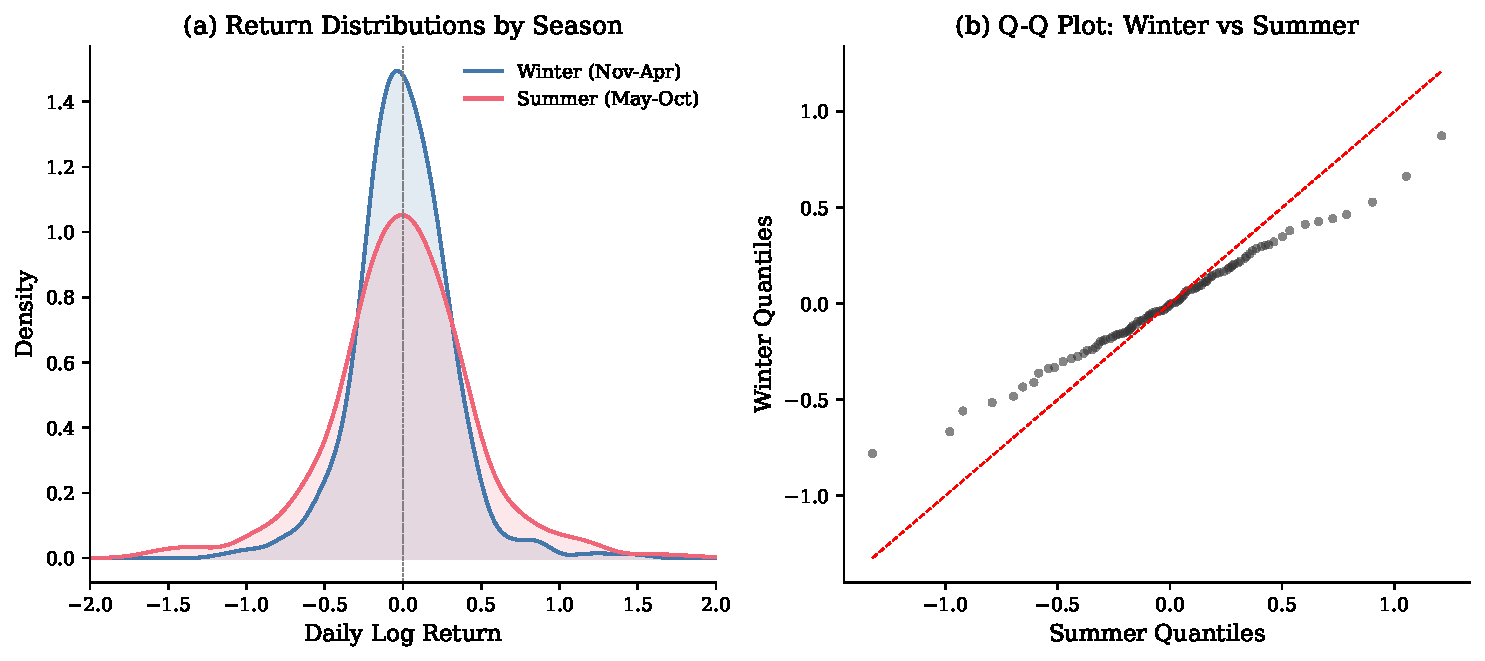
\includegraphics[width=0.85\textwidth]{figures/fig2_seasonal_distributions.pdf}
\caption{Distribution of daily NFT returns by season (winter: November--April; summer: May--October). Summer returns exhibit greater dispersion (standard deviation 44.4\% vs.\ 30.2\%), confirmed by the Levene test ($p < 0.001$). The distributions overlap substantially in location but differ markedly in scale.}\label{fig:seasonal_distributions}
\end{figure}

\subsection{Year-by-Year Decomposition}

Table~\ref{tab:year_by_year} reports the Halloween coefficient by cycle. The sign reversal across cycles (positive in 2020--2021, negative in 2021--2022 when fully controlled) with both coefficients individually insignificant confirms that the aggregate null does not mask offsetting sub-period effects.

\begin{table}[htbp]
\centering
\begin{threeparttable}
\caption{Year-by-Year Halloween Effect}
\label{tab:year_by_year}

\begin{tabular*}{\textwidth}{@{\extracolsep{\fill}} lcccc}
\toprule
Cycle & Winter mean & Summer mean & Diff. & $p$-value \\
\midrule
2020--2021 & 0.0127  & 0.0078   & +0.0049 & 0.892 \\
2021--2022 & -0.0036 & -0.0117  & +0.0081 & 0.776 \\
\bottomrule
\end{tabular*}

\begin{tablenotes}[flushleft]
\footnotesize
\item \textit{Notes:} Mean daily log returns by season within each Halloween year. $p$-values are from two-sided Welch $t$-tests. The 2020--2021 cycle covers November 2020--October 2021; the 2021--2022 cycle covers November 2021--October 2022.
\end{tablenotes}

\end{threeparttable}
\end{table}

\begin{figure}[htbp]
\centering
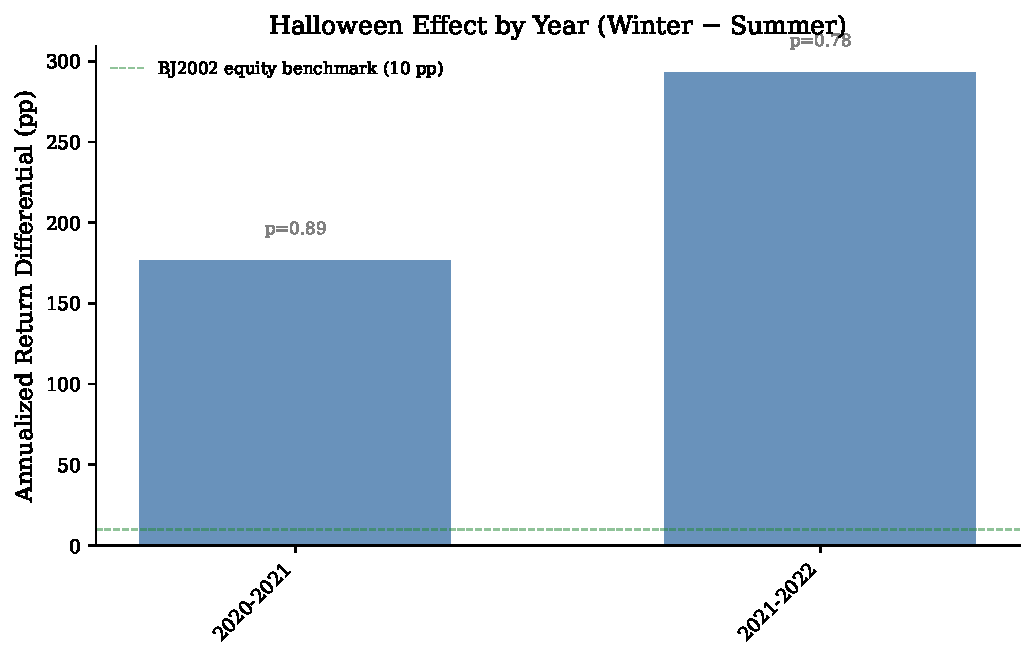
\includegraphics[width=0.85\textwidth]{figures/fig4_year_by_year.pdf}
\caption{Halloween effect by cycle: mean daily returns in winter and summer for each complete Halloween year. The sign of the winter--summer differential reverses across cycles, with neither difference statistically significant. Error bars represent 95\% confidence intervals.}\label{fig:year_by_year}
\end{figure}

Figure~\ref{fig:year_by_year} visualizes the seasonal return differential by cycle.

\subsection{Power Analysis}

Figure~\ref{fig:power_curve} displays the statistical power curve. Power to detect the equity-market Halloween benchmark (ten percentage points annualized) is approximately 5\%, indistinguishable from the size of the test. The minimum detectable effect at 80\% power is 1,150 basis points annualized, approximately 69 times the equity-market benchmark. This means the null result is informative about extreme seasonality (effects exceeding 1,000 basis points) but cannot address whether an economically meaningful Halloween effect of the magnitude found in equities exists in NFT markets. Longer time series are required to resolve this question.

\begin{figure}[htbp]
\centering
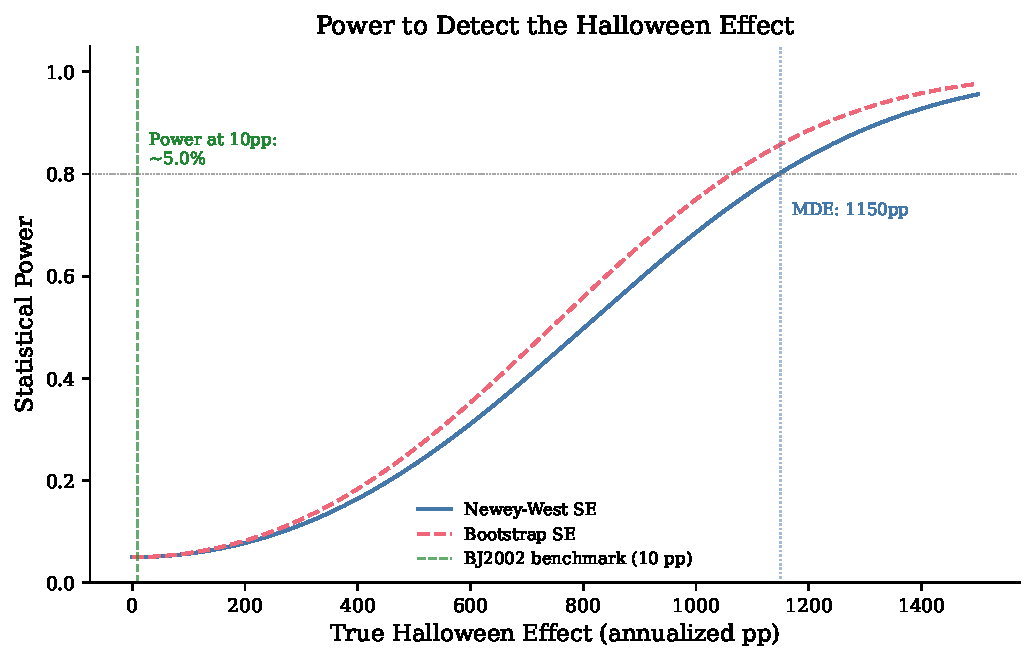
\includegraphics[width=0.85\textwidth]{figures/fig5_power_curve.pdf}
\caption{Statistical power as a function of the hypothesized annualized Halloween effect (basis points). The dashed vertical line marks the equity-market benchmark of approximately 10 percentage points from \citet{BoumanJacobsen2002}. At this magnitude, power is approximately 5\%, equal to the test size. The minimum detectable effect at 80\% power exceeds 1,150 basis points.}\label{fig:power_curve}
\end{figure}


% ══════════════════════════════════════════════════════════════════════
% 6. CROSS-SECTIONAL ANALYSIS
% ══════════════════════════════════════════════════════════════════════

\section{Cross-Sectional Analysis}\label{sec:crosssection}

\subsection{Day-of-Week Effects}

While six-month seasonality is absent, day-of-week effects are highly significant. The joint $F$-test for day-of-week indicators yields $F = 8.30$ ($p < 0.001$). Thursday and Friday returns are significantly negative relative to Sunday, with estimated differentials of $-$13.7 and $-$16.0 percentage points daily, respectively ($p < 0.001$ for both). Saturday returns are also significantly lower than Sunday ($p = 0.024$). This within-week calendar pattern mirrors the ``weekend effect'' documented in cryptocurrency markets by \citet{AharonQadan2019} and \citet{CaporalePlastun2019}, and it serves as a positive control: the data can detect calendar effects when they exist, strengthening confidence that the null result for the Halloween effect reflects a genuine absence rather than inadequate data quality. Figure~\ref{fig:calendar_effects} displays the day-of-week and month-of-year effects.

\begin{figure}[htbp]
\centering
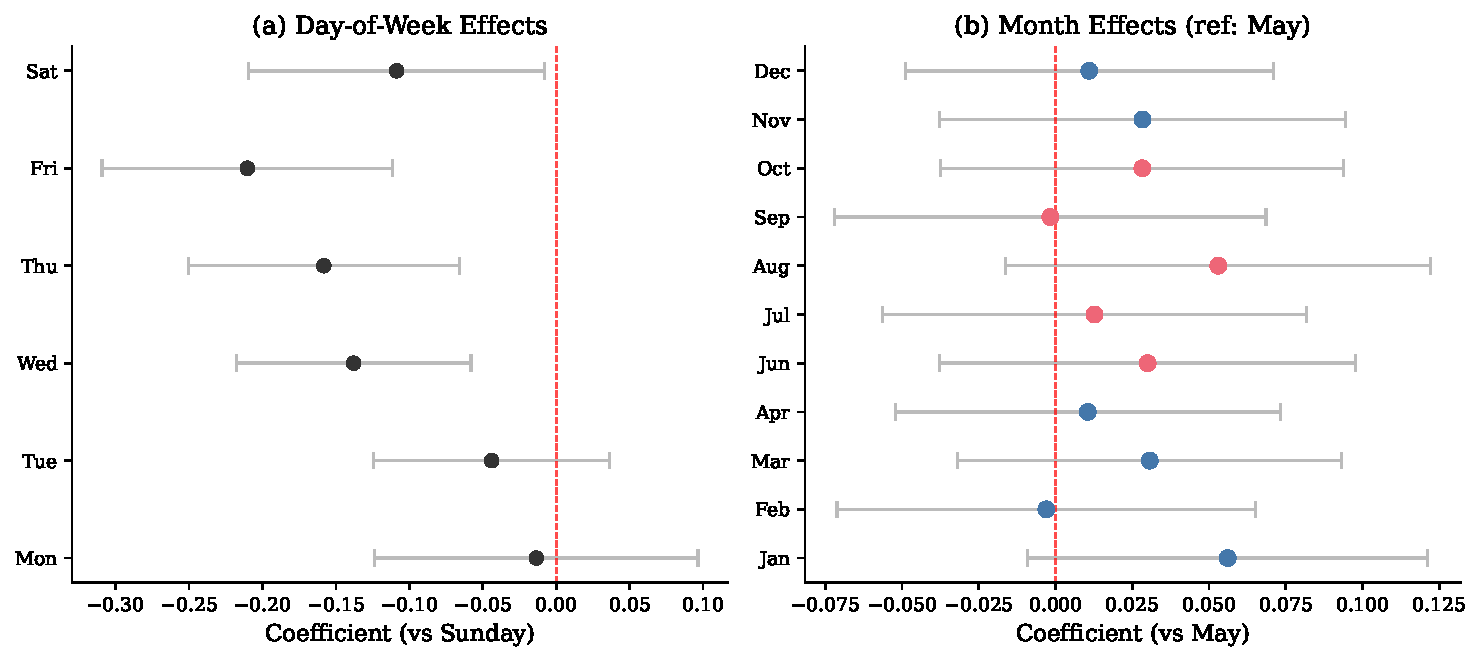
\includegraphics[width=0.85\textwidth]{figures/fig7_calendar_effects.pdf}
\caption{Day-of-week and month-of-year effects on daily NFT returns. The left panel shows that day-of-week effects are statistically significant (joint $F = 8.30$, $p < 0.001$), with Thursday through Saturday showing substantially lower returns than Sunday. The right panel shows no systematic monthly pattern.}\label{fig:calendar_effects}
\end{figure}

\subsection{January Effect}

A marginally significant January premium of 3.9 percentage points daily ($p = 0.029$) emerges from month-dummy regressions. The implied annualized magnitude (approximately 1,400 basis points for January alone) is economically implausible as a persistent anomaly and should be interpreted cautiously given the multiple-comparison problem inherent in testing twelve monthly dummies simultaneously. Applying a Bonferroni correction renders the January effect insignificant.

\subsection{Volume Seasonality}

Winter trading volume exceeds summer volume by a factor of 4.7, but this differential is not statistically significant ($p = 0.32$) in a regression of log volume on the Halloween indicator. The volume pattern is consistent with the attention hypothesis (higher winter engagement) but does not translate into detectable return seasonality. This decoupling between volume and return seasonality is diagnostic: it suggests that seasonal variation in market activity exists but does not generate predictable return differentials in the absence of institutional amplification mechanisms.

\subsection{Rolling Window Estimates}

Figure~\ref{fig:rolling} plots the Halloween coefficient from rolling 180-day windows. Of 806 windows, only 0.4\% produce a significant coefficient at the 5\% level, approximately what would be expected under the null by chance alone. The coefficient oscillates around zero with no persistent directional pattern, ruling out the possibility that a stable seasonal effect is masked by a specific sub-period.

\begin{figure}[htbp]
\centering
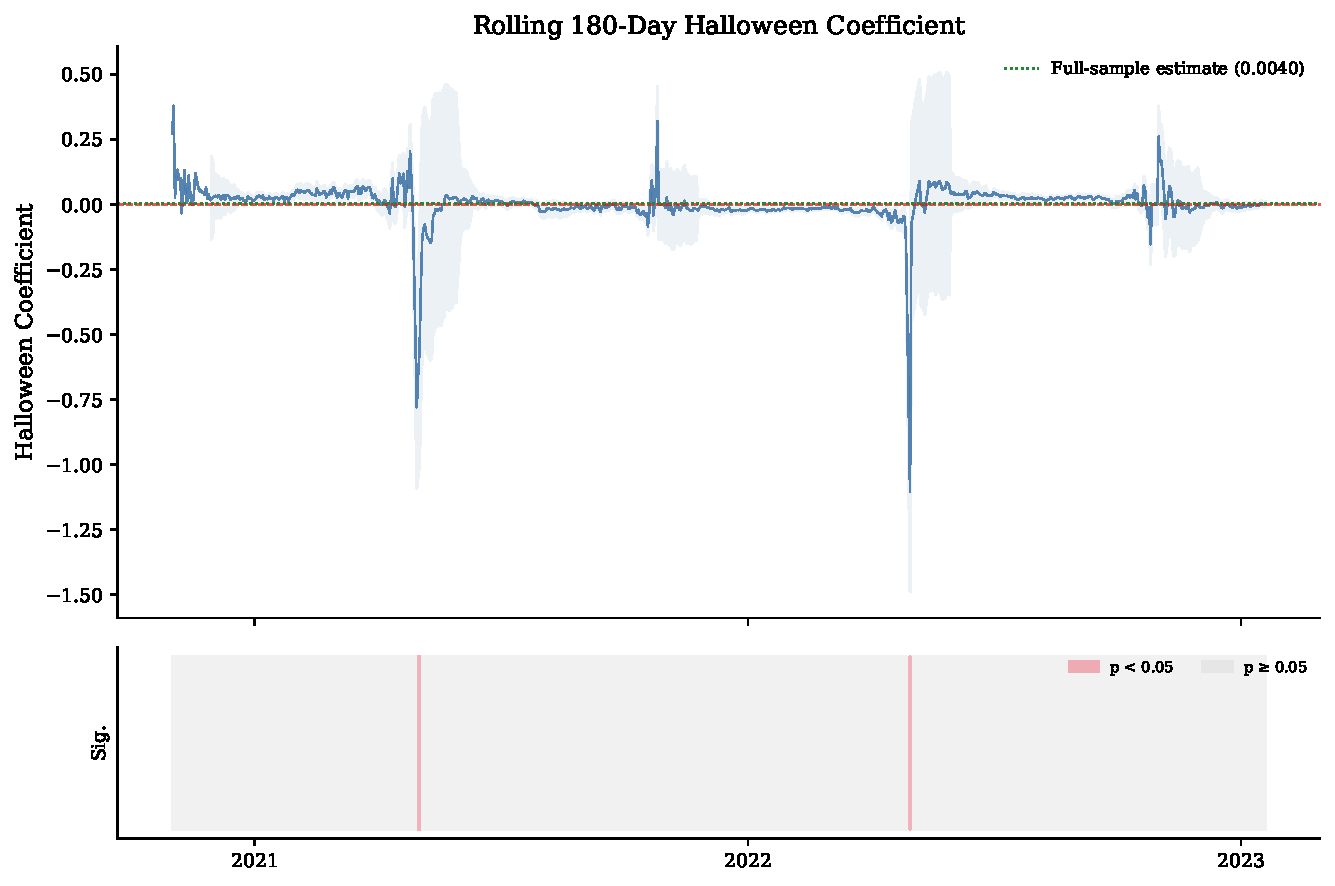
\includegraphics[width=0.85\textwidth]{figures/fig3_rolling_halloween.pdf}
\caption{Rolling 180-day Halloween coefficient estimates over the sample period. The shaded band represents the 95\% confidence interval. Only 0.4\% of windows produce a statistically significant coefficient, consistent with the expected false positive rate under the null hypothesis.}\label{fig:rolling}
\end{figure}


% ══════════════════════════════════════════════════════════════════════
% 7. ROBUSTNESS CHECKS
% ══════════════════════════════════════════════════════════════════════

\section{Robustness Checks}\label{sec:robustness}

Table~\ref{tab:robustness} summarizes the results of ten robustness checks. All confirm the null result. The block bootstrap (10,000 replications, 21-day blocks) yields a $p$-value of 0.719, with a 95\% confidence interval of [$-$0.016, 0.025] for the daily coefficient. The permutation test (10,000 reassignments) produces a supplementary $p$-value of 0.873; the discrepancy from the bootstrap reflects the violation of exchangeability documented in the diagnostics.

\begin{table}[htbp]
\centering
\begin{threeparttable}
\caption{Robustness Checks}
\label{tab:robustness}

\begin{tabular*}{\textwidth}{@{\extracolsep{\fill}} lccc}
\toprule
Check & $\hat{\beta}$ & $p$-value & Conclusion \\
\midrule
Block bootstrap (21-day, 10K)        & 0.0040  & 0.719   & Null confirmed \\
Permutation test (10K)               & 0.0040  & 0.873   & Null confirmed \\
Winsorized (1st/99th pctile)         & 0.0002  & 0.983   & Coefficient $\to 0$ \\
High-volume days ($>75$th pctile)    & -0.0213 & 0.216   & Sign reversal \\
Drop 2020                            & 0.0042  & 0.720   & Null holds \\
Drop 2021                            & 0.0071  & 0.605   & Null holds \\
Drop 2022                            & 0.0030  & 0.848   & Null holds \\
Drop 2023                            & 0.0029  & 0.801   & Null holds \\
Monthly frequency ($N=33$)           & 0.248   & 0.095   & See Table~\ref{tab:monthly} \\
Halloween $\times$ Year interaction  & ---     & $F=0.93$ & No time variation \\
\bottomrule
\end{tabular*}

\begin{tablenotes}[flushleft]
\footnotesize
\item \textit{Notes:} Block bootstrap uses stationary blocks of 21 days with 10,000 replications. The permutation test randomly reassigns months to winter and summer 10,000 times. Winsorization replaces returns below the 1st percentile and above the 99th percentile with the corresponding boundary values. Drop-year checks re-estimate the baseline excluding all observations from the specified year. The monthly specification uses 33 monthly observations; see Table~\ref{tab:monthly} for the full monthly analysis. All specifications use Newey--West standard errors except where noted.
\end{tablenotes}

\end{threeparttable}
\end{table}

Winsorization at the 1st and 99th percentiles shrinks the coefficient to near zero ($\hat{\beta} = 0.0002$, $p = 0.98$), indicating that the already-insignificant point estimate is driven by extreme return observations rather than a systematic seasonal shift in the return distribution. Restricting to high-volume days (above the 75th percentile) reverses the sign ($\hat{\beta} = -0.021$, $p = 0.22$), further undermining the robustness of any positive winter premium.

The drop-one-year jackknife confirms that no single year drives the result: the coefficient remains insignificant regardless of which year is excluded, with $p$-values ranging from 0.61 to 0.85. At monthly frequency ($N = 33$), the coefficient is larger ($\hat{\beta} = 0.248$, $p = 0.095$) and reaches significance with ETH controls ($p = 0.049$); Section~\ref{sec:frequency} provides a detailed analysis of this frequency sensitivity and explains why the monthly result does not overturn the daily null. The Halloween-by-year interaction $F$-test ($F = 0.93$) cannot reject constant seasonal effects across years, though this is unsurprising given the low power.

Figure~\ref{fig:coefficient_comparison} visualizes the Halloween coefficient and its confidence interval across all four main specifications, illustrating the sign instability and the width of the confidence bands relative to the equity benchmark.

\begin{figure}[htbp]
\centering
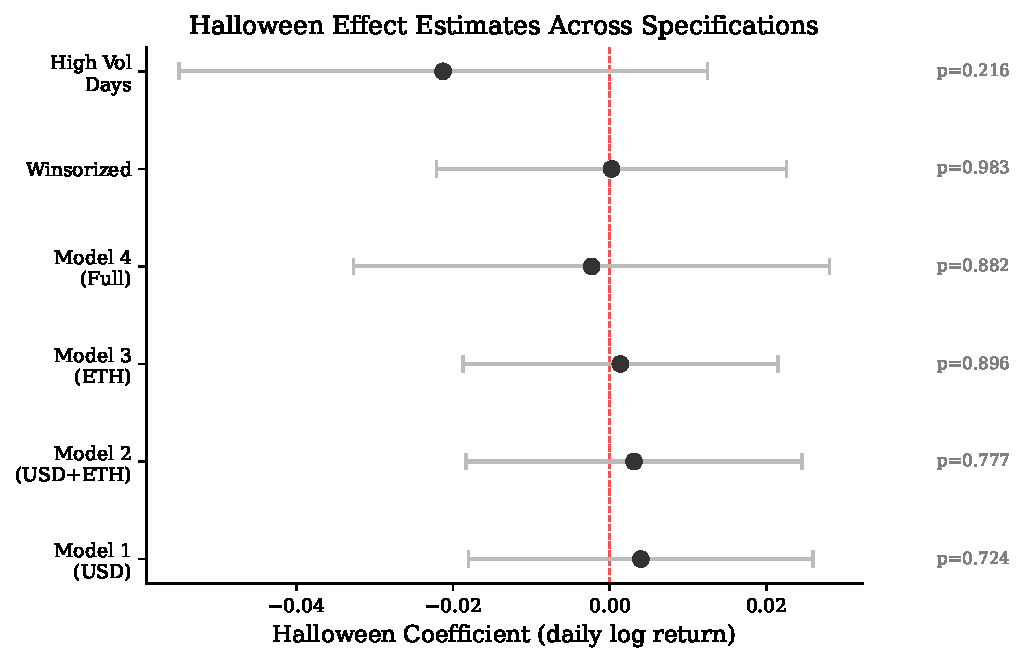
\includegraphics[width=0.85\textwidth]{figures/fig1_coefficient_comparison.pdf}
\caption{Halloween coefficient estimates across the four main specifications (Table~\ref{tab:main_results}). Points indicate $\hat{\beta}$; bars indicate 95\% Newey-West confidence intervals. The coefficient is insignificant in all specifications and reverses sign in the full model.}\label{fig:coefficient_comparison}
\end{figure}

Figure~\ref{fig:bootstrap} displays the bootstrap distribution of the Halloween coefficient from 10,000 block bootstrap replications. The observed coefficient (vertical line) falls well within the body of the null distribution, consistent with no seasonal effect.

\begin{figure}[htbp]
\centering
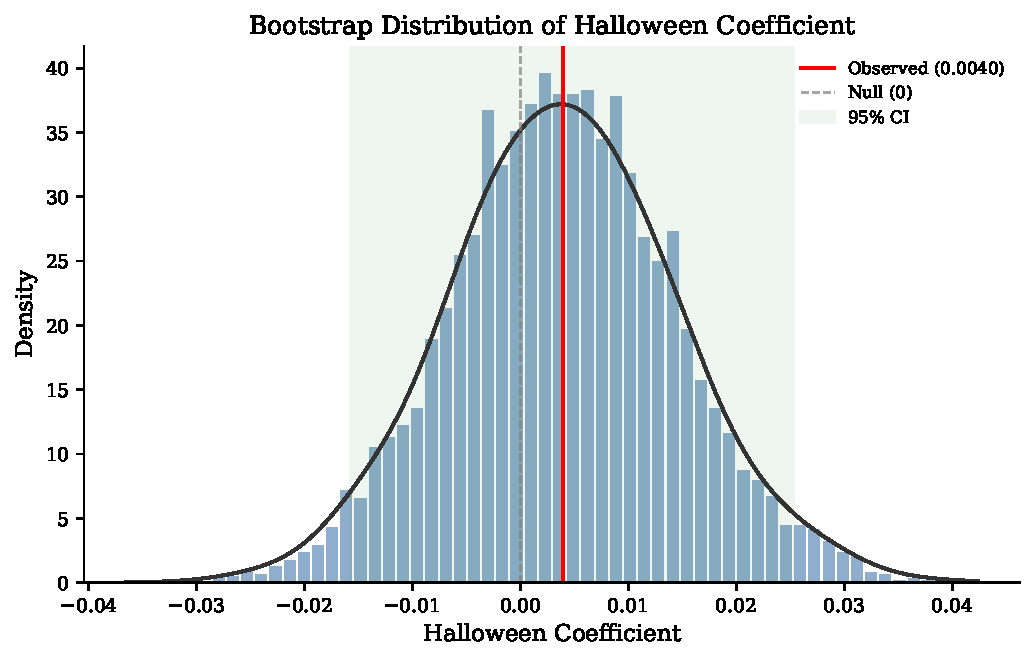
\includegraphics[width=0.85\textwidth]{figures/fig6_bootstrap_distribution.pdf}
\caption{Bootstrap distribution of the Halloween coefficient from 10,000 block bootstrap replications with 21-day blocks. The vertical dashed line marks the observed coefficient ($\hat{\beta} = 0.0040$). The distribution is centered near zero, and the observed value falls well within the 95\% interval.}\label{fig:bootstrap}
\end{figure}


% ══════════════════════════════════════════════════════════════════════
% 8. DISCUSSION
% ══════════════════════════════════════════════════════════════════════

\section{Discussion}\label{sec:discussion}

\subsection{Summary and Interpretation}

The Halloween effect, the most persistent calendar anomaly in equity markets, does not extend to NFT markets. Across four regression specifications, two denomination schemes, ten robustness checks, and year-by-year decompositions, we find no statistically or economically significant seasonal return differential. The raw USD-denominated point estimate of 145 basis points annualized is dominated by ETH price pass-through (66\%), and the NFT-specific residual of 49 basis points is indistinguishable from noise. The coefficient is unstable across specifications, flipping sign under full controls, and is driven by extreme returns that vanish under winsorization.

The absence of the anomaly in a market structurally stripped of institutional features is consistent with a reading where institutional mechanisms play a necessary, though perhaps not sufficient, role in generating the equity Halloween effect. Equity markets combine institutional calendar-linked flows (fiscal-year rebalancing, mutual fund window-dressing, earnings announcement clustering) with behavioral channels (seasonal mood, vacation-driven inattention). NFT markets preserve the behavioral channels while eliminating the institutional ones. The null result suggests that behavioral forces alone do not generate a detectable six-month seasonal pattern in returns, at least at the volatility levels and sample sizes characteristic of emerging digital asset markets.

\subsection{Theoretical Implications}

The findings bear on the mechanism debate in three ways. First, the result challenges pure behavioral explanations of the Halloween effect. If seasonal mood shifts \citep{KamstraKramerLevi2003} or vacation-induced inattention \citep{HongYu2009} were sufficient to generate the anomaly, the effect should appear in NFT markets, where the overwhelmingly retail participant base is directly exposed to these psychological channels without institutional intermediation. The absence of the effect, subject to the power caveat discussed below, is more consistent with models in which institutional trading patterns interact with behavioral tendencies to produce the observed seasonal regularity.

Second, the finding that volume seasonality exists (winter volume exceeds summer by a factor of 2.7) without accompanying return seasonality provides a new stylized fact for models of calendar anomalies. In \citet{HongYu2009}, reduced summer participation depresses returns; our data show a qualitatively similar participation pattern (higher winter engagement) that does not translate into return differentials. One interpretation is that in the absence of institutional amplification, behavioral variation in market activity is insufficient to move equilibrium prices. Another is that the volume pattern itself reflects composition effects (larger trades in winter) rather than more participants, weakening the link between the attention channel and return predictability.

Third, the strong day-of-week effects provide a calibration benchmark. NFT markets exhibit significant within-week return patterns (Thursday and Friday substantially below Sunday), consistent with the cryptocurrency weekend effect. The coexistence of significant day-of-week effects and insignificant seasonal effects suggests that calendar anomalies transfer to NFT markets at short horizons but not at the six-month frequency. This horizon dependence is consistent with attention-based models in which short-term behavioral rhythms (weekly routines) are more regular than long-term ones (seasonal patterns), or with market microstructure explanations in which weekly liquidity cycles generate predictable return patterns while seasonal liquidity variation does not.

\subsection{Practical Implications}

The results have straightforward implications for NFT market participants and platform designers. Seasonal trading strategies based on the ``Sell in May'' heuristic are not supported by the data. Even the point estimate of the winter premium (145 basis points annualized in USD) falls well below the round-trip transaction costs on NFT platforms (approximately 5\% in platform fees alone, before gas costs). No specification produces an effect large enough to survive implementation costs.

For platform designers, the significant day-of-week effects suggest that within-week liquidity management may be more consequential than seasonal considerations. Platforms could optimize fee structures or promotional activities around the observed weekly pattern rather than seasonal cycles. The variance seasonality finding (summer returns 2.2 times more volatile) may be relevant for risk management and margin-setting on NFT lending protocols, though the pattern likely reflects the specific historical trajectory of the 2021 boom-bust cycle rather than a stable structural feature.

\subsection{Limitations}

The most binding limitation is statistical power. With 990 daily observations spanning approximately 2.7 years, the test has only 5\% power to detect an equity-magnitude Halloween effect (ten percentage points annualized). The minimum detectable effect at 80\% power exceeds 1,100 basis points. The null result therefore rules out extreme seasonality but cannot exclude economically meaningful effects at the scale documented in equities. Longer NFT market time series, which will become available as the market matures, are required to resolve whether a smaller but genuine Halloween effect exists.

The portfolio construction method introduces potential biases. The mean-price-based index equal-weights active collections, overrepresenting small and illiquid NFTs relative to market capitalization. A value-weighted index or a repeat-sale index would better reflect the experience of a representative investor, but both require row-level trade data that was not available in the current pipeline run.

Cross-sectional analysis at the platform and collection-tier level was infeasible in this run due to data availability constraints. Tests of whether incentivized platforms (LooksRare, X2Y2) exhibit different seasonal patterns than organic platforms (OpenSea), or whether blue-chip collections show different seasonality than long-tail collections, remain priorities for future work. These tests could reveal whether the aggregate null masks offsetting effects across market segments.

The wash trade exclusion relies solely on same-wallet buyer-seller matches, capturing 0.025\% of trades. More sophisticated detection methods (circular trading chains, zero-profit round-trips, same-block trading) could not be applied without row-level data. If wash trading exhibits seasonal patterns tied to token reward schedules, the measured returns on incentivized platforms may be distorted in ways that the self-trade filter does not address.

The retail attention channel, a key theoretical mechanism, remains untested. Google Trends data for NFT-related search queries was not incorporated. Future work incorporating attention proxies could test whether the volume seasonality documented here operates through the attention channel and whether attention seasonality predicts return seasonality conditional on institutional features.

\subsection{Future Research}

Three directions emerge from these findings. First, as the NFT market accumulates additional years of trading history, re-testing the Halloween effect with greater statistical power is a natural extension. The minimum detectable effect will shrink roughly in proportion to the square root of the number of additional seasonal cycles, and a sample spanning five to seven complete cycles would substantially improve the ability to detect equity-magnitude effects.

Second, the variance seasonality finding (summer returns 2.2 times more volatile than winter) warrants investigation as a potential stylized fact of NFT market dynamics. If the pattern persists beyond the 2021 boom-bust episode, it may reflect a structural feature of retail-dominated digital asset markets in which speculative activity and attention concentrate in specific calendar periods, generating volatility clustering without predictable return differentials. Connecting this variance pattern to the \citet{DimpflJank2016} framework, which links attention fluctuations to volatility, could yield new theoretical insights.

Third, comparing the Halloween effect across digital asset classes at different points on the institutional participation spectrum (Bitcoin, which has substantial institutional investment; Ethereum, with moderate institutional presence; and NFTs, with minimal institutional involvement) would directly test whether the gradient of institutional participation maps onto the gradient of seasonal return anomalies.


% ══════════════════════════════════════════════════════════════════════
% 9. CONCLUSION
% ══════════════════════════════════════════════════════════════════════

\section{Conclusion}\label{sec:conclusion}

This paper tests whether the Halloween effect, the most robust calendar anomaly in equity markets, extends to NFT markets. Using 35.8 million trades across eight platforms from 2017 to 2023, we find no statistically significant seasonal return differential. The raw USD-denominated winter premium is a pass-through of ETH price seasonality, and the NFT-specific component in ETH denomination is economically and statistically negligible. The result holds across all specifications and robustness checks.

The absence of the Halloween effect in a market without institutional investors, short selling, or exchange closures is consistent with institutional mechanisms playing a necessary role in sustaining the equity anomaly. Behavioral channels operating through retail investor psychology do not generate a detectable six-month seasonal pattern in NFT returns, though this conclusion must be qualified by the severe power constraint imposed by the short sample.

Two novel findings complement the main result. Summer NFT returns are 2.2 times more volatile than winter returns, a significant asymmetry that warrants further investigation as the market matures. Day-of-week effects are highly significant, suggesting that within-week calendar regularities transfer to digital collectible markets even when longer-horizon seasonal patterns do not. Together, these results contribute to the growing body of evidence on return dynamics in emerging digital asset classes and provide new evidence on the mechanisms underlying the most enduring calendar anomaly in finance.





% ══════════════════════════════════════════════════════════════════════
% REFERENCES
% ══════════════════════════════════════════════════════════════════════

\FloatBarrier

\bibliographystyle{plainnat}
\bibliography{references}

\end{document}
